% Options for packages loaded elsewhere
\PassOptionsToPackage{unicode}{hyperref}
\PassOptionsToPackage{hyphens}{url}
%
\documentclass[
]{article}
\usepackage{amsmath,amssymb}
\usepackage{iftex}
\ifPDFTeX
  \usepackage[T1]{fontenc}
  \usepackage[utf8]{inputenc}
  \usepackage{textcomp} % provide euro and other symbols
\else % if luatex or xetex
  \usepackage{unicode-math} % this also loads fontspec
  \defaultfontfeatures{Scale=MatchLowercase}
  \defaultfontfeatures[\rmfamily]{Ligatures=TeX,Scale=1}
\fi
\usepackage{lmodern}
\ifPDFTeX\else
  % xetex/luatex font selection
\fi
% Use upquote if available, for straight quotes in verbatim environments
\IfFileExists{upquote.sty}{\usepackage{upquote}}{}
\IfFileExists{microtype.sty}{% use microtype if available
  \usepackage[]{microtype}
  \UseMicrotypeSet[protrusion]{basicmath} % disable protrusion for tt fonts
}{}
\makeatletter
\@ifundefined{KOMAClassName}{% if non-KOMA class
  \IfFileExists{parskip.sty}{%
    \usepackage{parskip}
  }{% else
    \setlength{\parindent}{0pt}
    \setlength{\parskip}{6pt plus 2pt minus 1pt}}
}{% if KOMA class
  \KOMAoptions{parskip=half}}
\makeatother
\usepackage{xcolor}
\usepackage{color}
\usepackage{fancyvrb}
\newcommand{\VerbBar}{|}
\newcommand{\VERB}{\Verb[commandchars=\\\{\}]}
\DefineVerbatimEnvironment{Highlighting}{Verbatim}{commandchars=\\\{\}}
% Add ',fontsize=\small' for more characters per line
\newenvironment{Shaded}{}{}
\newcommand{\AlertTok}[1]{\textcolor[rgb]{1.00,0.00,0.00}{\textbf{#1}}}
\newcommand{\AnnotationTok}[1]{\textcolor[rgb]{0.38,0.63,0.69}{\textbf{\textit{#1}}}}
\newcommand{\AttributeTok}[1]{\textcolor[rgb]{0.49,0.56,0.16}{#1}}
\newcommand{\BaseNTok}[1]{\textcolor[rgb]{0.25,0.63,0.44}{#1}}
\newcommand{\BuiltInTok}[1]{\textcolor[rgb]{0.00,0.50,0.00}{#1}}
\newcommand{\CharTok}[1]{\textcolor[rgb]{0.25,0.44,0.63}{#1}}
\newcommand{\CommentTok}[1]{\textcolor[rgb]{0.38,0.63,0.69}{\textit{#1}}}
\newcommand{\CommentVarTok}[1]{\textcolor[rgb]{0.38,0.63,0.69}{\textbf{\textit{#1}}}}
\newcommand{\ConstantTok}[1]{\textcolor[rgb]{0.53,0.00,0.00}{#1}}
\newcommand{\ControlFlowTok}[1]{\textcolor[rgb]{0.00,0.44,0.13}{\textbf{#1}}}
\newcommand{\DataTypeTok}[1]{\textcolor[rgb]{0.56,0.13,0.00}{#1}}
\newcommand{\DecValTok}[1]{\textcolor[rgb]{0.25,0.63,0.44}{#1}}
\newcommand{\DocumentationTok}[1]{\textcolor[rgb]{0.73,0.13,0.13}{\textit{#1}}}
\newcommand{\ErrorTok}[1]{\textcolor[rgb]{1.00,0.00,0.00}{\textbf{#1}}}
\newcommand{\ExtensionTok}[1]{#1}
\newcommand{\FloatTok}[1]{\textcolor[rgb]{0.25,0.63,0.44}{#1}}
\newcommand{\FunctionTok}[1]{\textcolor[rgb]{0.02,0.16,0.49}{#1}}
\newcommand{\ImportTok}[1]{\textcolor[rgb]{0.00,0.50,0.00}{\textbf{#1}}}
\newcommand{\InformationTok}[1]{\textcolor[rgb]{0.38,0.63,0.69}{\textbf{\textit{#1}}}}
\newcommand{\KeywordTok}[1]{\textcolor[rgb]{0.00,0.44,0.13}{\textbf{#1}}}
\newcommand{\NormalTok}[1]{#1}
\newcommand{\OperatorTok}[1]{\textcolor[rgb]{0.40,0.40,0.40}{#1}}
\newcommand{\OtherTok}[1]{\textcolor[rgb]{0.00,0.44,0.13}{#1}}
\newcommand{\PreprocessorTok}[1]{\textcolor[rgb]{0.74,0.48,0.00}{#1}}
\newcommand{\RegionMarkerTok}[1]{#1}
\newcommand{\SpecialCharTok}[1]{\textcolor[rgb]{0.25,0.44,0.63}{#1}}
\newcommand{\SpecialStringTok}[1]{\textcolor[rgb]{0.73,0.40,0.53}{#1}}
\newcommand{\StringTok}[1]{\textcolor[rgb]{0.25,0.44,0.63}{#1}}
\newcommand{\VariableTok}[1]{\textcolor[rgb]{0.10,0.09,0.49}{#1}}
\newcommand{\VerbatimStringTok}[1]{\textcolor[rgb]{0.25,0.44,0.63}{#1}}
\newcommand{\WarningTok}[1]{\textcolor[rgb]{0.38,0.63,0.69}{\textbf{\textit{#1}}}}
\usepackage{longtable,booktabs,array}
\usepackage{calc} % for calculating minipage widths
% Correct order of tables after \paragraph or \subparagraph
\usepackage{etoolbox}
\makeatletter
\patchcmd\longtable{\par}{\if@noskipsec\mbox{}\fi\par}{}{}
\makeatother
% Allow footnotes in longtable head/foot
\IfFileExists{footnotehyper.sty}{\usepackage{footnotehyper}}{\usepackage{footnote}}
\makesavenoteenv{longtable}
\usepackage{graphicx}
\makeatletter
\def\maxwidth{\ifdim\Gin@nat@width>\linewidth\linewidth\else\Gin@nat@width\fi}
\def\maxheight{\ifdim\Gin@nat@height>\textheight\textheight\else\Gin@nat@height\fi}
\makeatother
% Scale images if necessary, so that they will not overflow the page
% margins by default, and it is still possible to overwrite the defaults
% using explicit options in \includegraphics[width, height, ...]{}
\setkeys{Gin}{width=\maxwidth,height=\maxheight,keepaspectratio}
% Set default figure placement to htbp
\makeatletter
\def\fps@figure{htbp}
\makeatother
\ifLuaTeX
  \usepackage{luacolor}
  \usepackage[soul]{lua-ul}
\else
  \usepackage{soul}
\fi
\setlength{\emergencystretch}{3em} % prevent overfull lines
\providecommand{\tightlist}{%
  \setlength{\itemsep}{0pt}\setlength{\parskip}{0pt}}
\setcounter{secnumdepth}{-\maxdimen} % remove section numbering
\ifLuaTeX
  \usepackage{selnolig}  % disable illegal ligatures
\fi
\IfFileExists{bookmark.sty}{\usepackage{bookmark}}{\usepackage{hyperref}}
\IfFileExists{xurl.sty}{\usepackage{xurl}}{} % add URL line breaks if available
\urlstyle{same}
\hypersetup{
  hidelinks,
  pdfcreator={LaTeX via pandoc}}

\author{}
\date{}

\begin{document}

\hypertarget{alepvetux151-markdown-szintaxis}{%
\section{Alepvető Markdown
Szintaxis}\label{alepvetux151-markdown-szintaxis}}

\begin{quote}
Címek
\end{quote}

\hypertarget{h1}{%
\section{H1}\label{h1}}

\hypertarget{h2}{%
\subsection{H2}\label{h2}}

\hypertarget{h3}{%
\subsubsection{H3}\label{h3}}

\begin{center}\rule{0.5\linewidth}{0.5pt}\end{center}

\begin{quote}
Félkövér szöveg
\end{quote}

\textbf{félkövér text}

\begin{center}\rule{0.5\linewidth}{0.5pt}\end{center}

\begin{quote}
Dőlt szöveg
\end{quote}

\textbf{\emph{ez itt egy dőlt szöveg}}

\begin{center}\rule{0.5\linewidth}{0.5pt}\end{center}

\begin{quote}
Bloquote
\end{quote}

\begin{center}\rule{0.5\linewidth}{0.5pt}\end{center}

\begin{quote}
Számozott lista
\end{quote}

\begin{enumerate}
\def\labelenumi{\arabic{enumi}.}
\tightlist
\item
  Első elem
\item
  Második elem
\item
  Harmadik elem
\end{enumerate}

\begin{center}\rule{0.5\linewidth}{0.5pt}\end{center}

\begin{quote}
Számozatlan lista
\end{quote}

\begin{itemize}
\tightlist
\item
  Első elem
\item
  Második elem
\item
  Harmadik elem
\end{itemize}

\begin{center}\rule{0.5\linewidth}{0.5pt}\end{center}

\begin{quote}
Elkerített (\emph{fenced}) kódblokk (kiterjesztett szintaxis)
\end{quote}

\begin{Shaded}
\begin{Highlighting}[]
\KeywordTok{public} \DataTypeTok{static} \DataTypeTok{void} \FunctionTok{main}\OperatorTok{(}\BuiltInTok{String}\OperatorTok{[]}\NormalTok{ args}\OperatorTok{)} \OperatorTok{\{}
    \BuiltInTok{System}\OperatorTok{.}\FunctionTok{out}\OperatorTok{.}\FunctionTok{println}\OperatorTok{(}\StringTok{"Hello Világ!"}\OperatorTok{);}
\OperatorTok{\}}
\end{Highlighting}
\end{Shaded}

\begin{center}\rule{0.5\linewidth}{0.5pt}\end{center}

\begin{quote}
Beágyazott (inline) kód
\end{quote}

\texttt{System.out.println("Hello\ Világ!");}

\begin{center}\rule{0.5\linewidth}{0.5pt}\end{center}

\begin{quote}
Linkek
\end{quote}

\href{https://www.google.com}{Google}

\begin{center}\rule{0.5\linewidth}{0.5pt}\end{center}

\begin{quote}
Képek
\end{quote}

\begin{figure}
\centering
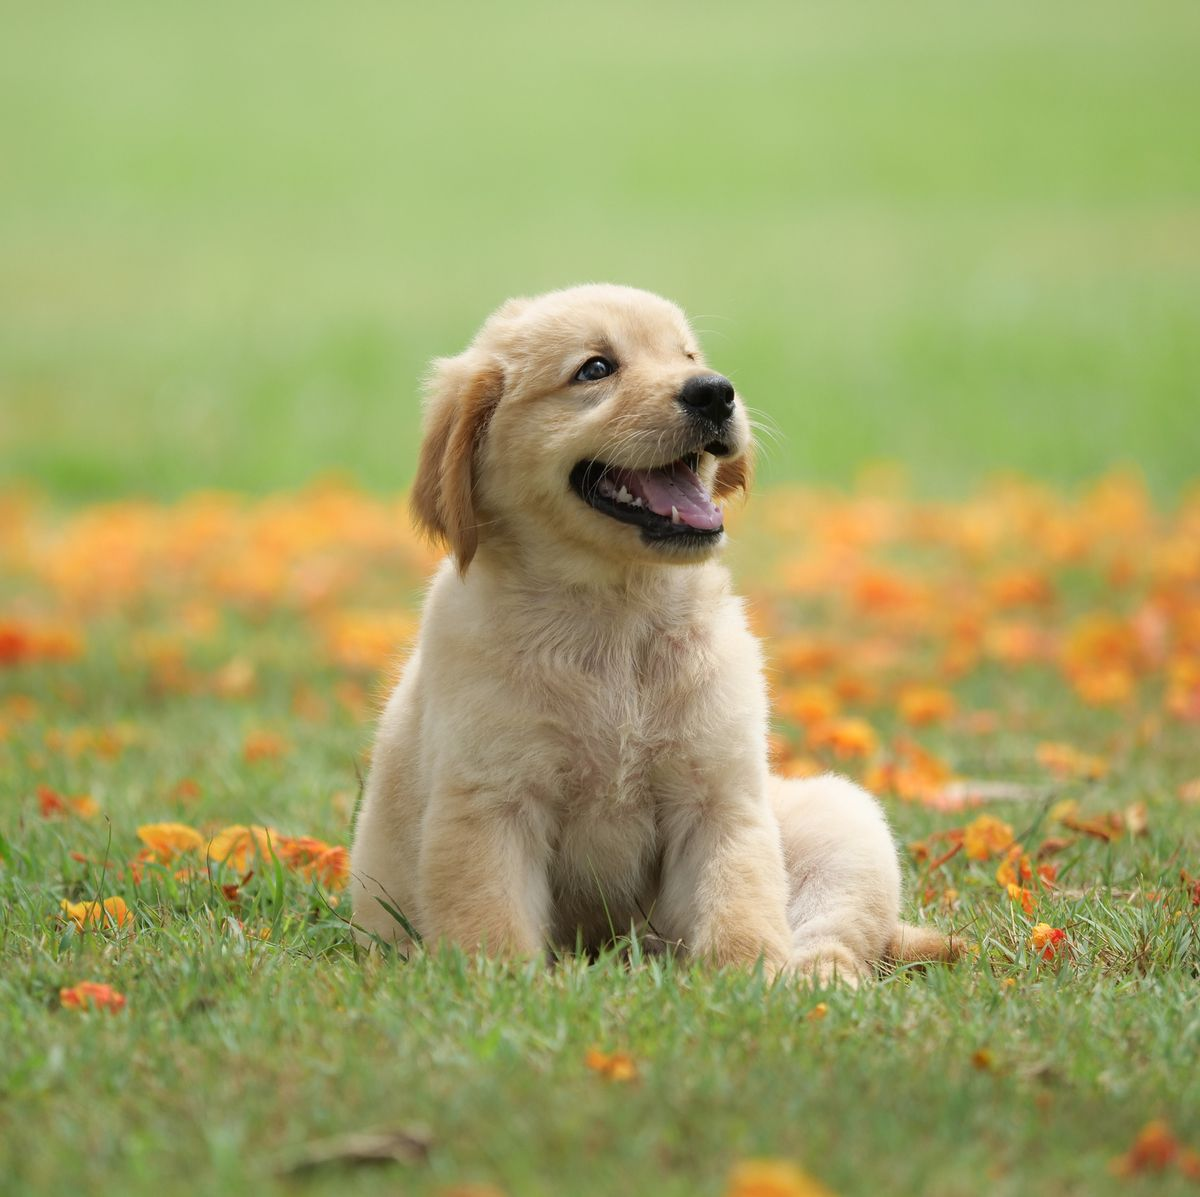
\includegraphics{dog.jpg}
\caption{Ez itt egy kutya.}
\end{figure}

\begin{center}\rule{0.5\linewidth}{0.5pt}\end{center}

\hypertarget{kiterjesztett-markdown-szintaxis}{%
\section{Kiterjesztett Markdown
Szintaxis}\label{kiterjesztett-markdown-szintaxis}}

\begin{quote}
Táblázatok
\end{quote}

\begin{longtable}[]{@{}ll@{}}
\toprule\noalign{}
Oszlop 1 & Oszlop 2 \\
\midrule\noalign{}
\endhead
\bottomrule\noalign{}
\endlastfoot
Sor 1 & Sor1 \\
Sor 2 & Sor 2 \\
\end{longtable}

\begin{center}\rule{0.5\linewidth}{0.5pt}\end{center}

\begin{quote}
Lábjegyzék
\end{quote}

Ez itt egy lábjegyzék. {[}\^{}1{]} {[}\^{}1{]}: Ez itt egy lábjegyzék.

\begin{center}\rule{0.5\linewidth}{0.5pt}\end{center}

\begin{quote}
Feladat/ellenőrző lista (\emph{todo/check list})
\end{quote}

\begin{itemize}
\tightlist
\item[$\boxtimes$]
  Tanulás
\item[$\square$]
  Kódolás
\item[$\square$]
  Takarítás
\end{itemize}

\begin{center}\rule{0.5\linewidth}{0.5pt}\end{center}

\begin{quote}
Szöveg áthúzás
\end{quote}

\st{A Föld lapos.}

\begin{center}\rule{0.5\linewidth}{0.5pt}\end{center}

\begin{quote}
Emoji
\end{quote}

Ez nagyon vicces! :joy:

\begin{center}\rule{0.5\linewidth}{0.5pt}\end{center}

\begin{quote}
Kijelölés
\end{quote}

Ki kell jelölnöm ezeket a ==nagyon fontos szavakat==.

\begin{center}\rule{0.5\linewidth}{0.5pt}\end{center}

\begin{quote}
Matematika
\end{quote}

\(f(x)=x^2+1\)

\begin{center}\rule{0.5\linewidth}{0.5pt}\end{center}

\begin{quote}
Alsó index (\emph{subscript})
\end{quote}

H\textsubscript{2}O

\begin{center}\rule{0.5\linewidth}{0.5pt}\end{center}

\begin{quote}
Felső index (\emph{superscript})
\end{quote}

X\textsuperscript{2}

\begin{center}\rule{0.5\linewidth}{0.5pt}\end{center}

\textbf{Forrás}:
\href{https://www.markdownguide.org/cheat-sheet/}{Markdown Cheatsheet}

\end{document}
